\section{Introduction}

\subsection{Motivation}

Computational algorithms described in scientific papers can be hard to grasp. A very common technique to help with understanding are visualizations in the form of sketches and diagrams, output tables to keep track of certain variables in the algorithm's execution, or arrows to indicate recursive calls.

However, these visualizations are usually limited by the constraints put on them by the typesetting system they are written in, which produces output to be printed on physical paper: they are static, they cover just one example or a very small and incomplete subset of possible examples, and they are often manually specified instead of generated from an already existing implementation of an algorithm. Furthermore, scientific journals even further broaden those constraints by imposing page or word limits on article submissions.

While it is possible to create graphical representations of data structures like graphs in a typesetting system such as \LaTeX  using libraries like \texttt{pgf-tikz}\footnote{\url{https://github.com/pgf-tikz/pgf}}, those are often cumbersome and time-consuming  to specify.


As media can be and are consumed digitally though on graphical user interfaces on the bitmap screen of a laptop or tablet computer, these limitations seem artificial and mostly stem from the ``printability'' aspect of the paper.


A further explanation for the lack of available visualizations is that instructors often don't have the time or resources to produce high-quality, interactive visualizations for their algorithms.

A common compromise is to use presentation software like Microsoft PowerPoint which comps  

While the 2002 publications from Hundhausen et al. \cite{hundhausen2002meta} and Naps et al. \cite{naps2002exploring} criticize the efficiacy of algorithm visualizations as a pedagogical tool, numerous successful examples have emerged in more recent years.
Hohman et al. present and discuss many of such examples in their 2020 article ``Communicating with Interactive Articles'' \cite{hohman2020communicating}.
The YouTube channel ``3blue1brown'' who specializes on the visualization of concepts in mathematics and computer science has gained 5 million subscribers in 4 years and is collaborating with a group at MIT to provide supplementary materials for their course on computational thinking \footnote{\url{https://www.patreon.com/posts/mit-lectures-41240316}}.


This thesis draws inspiration Python-based mathematics visualization library \texttt{manim}\footnote{https://github.com/3b1b/manim}.

\subsection{Goal of this Thesis}
to visualize algorithms from in specific instances.

The domain of query optimization poses many algorithms that can be visualized well.

However, visualizing algorithms can provide far more than just merely helping students understand the intricate concepts better.
Among professional computer scientists and software engineers the visualization of algorithms has proven a useful debugging and exploration technique.

In this Master thesis, I want to provide a generic toolset for algorithms. I aim for a framework that lets you generate the visualizations in a generic way—no explicit drawing is needed.

Instead of investigating what the constitutents of an algorithm \textit{could} be and
implementing them accordingly, we use a top-down approach and implement the steps of
two pre-chosen algorithms, namely \texttt{DPccp} \cite{moerkotte2006analysis} and Adaptive Radix Trees \cite{leis2013adaptive}.

Lack of good tooling in database algorithm development.
Visual debugging and aids more commonplace.
\begin{figure}
    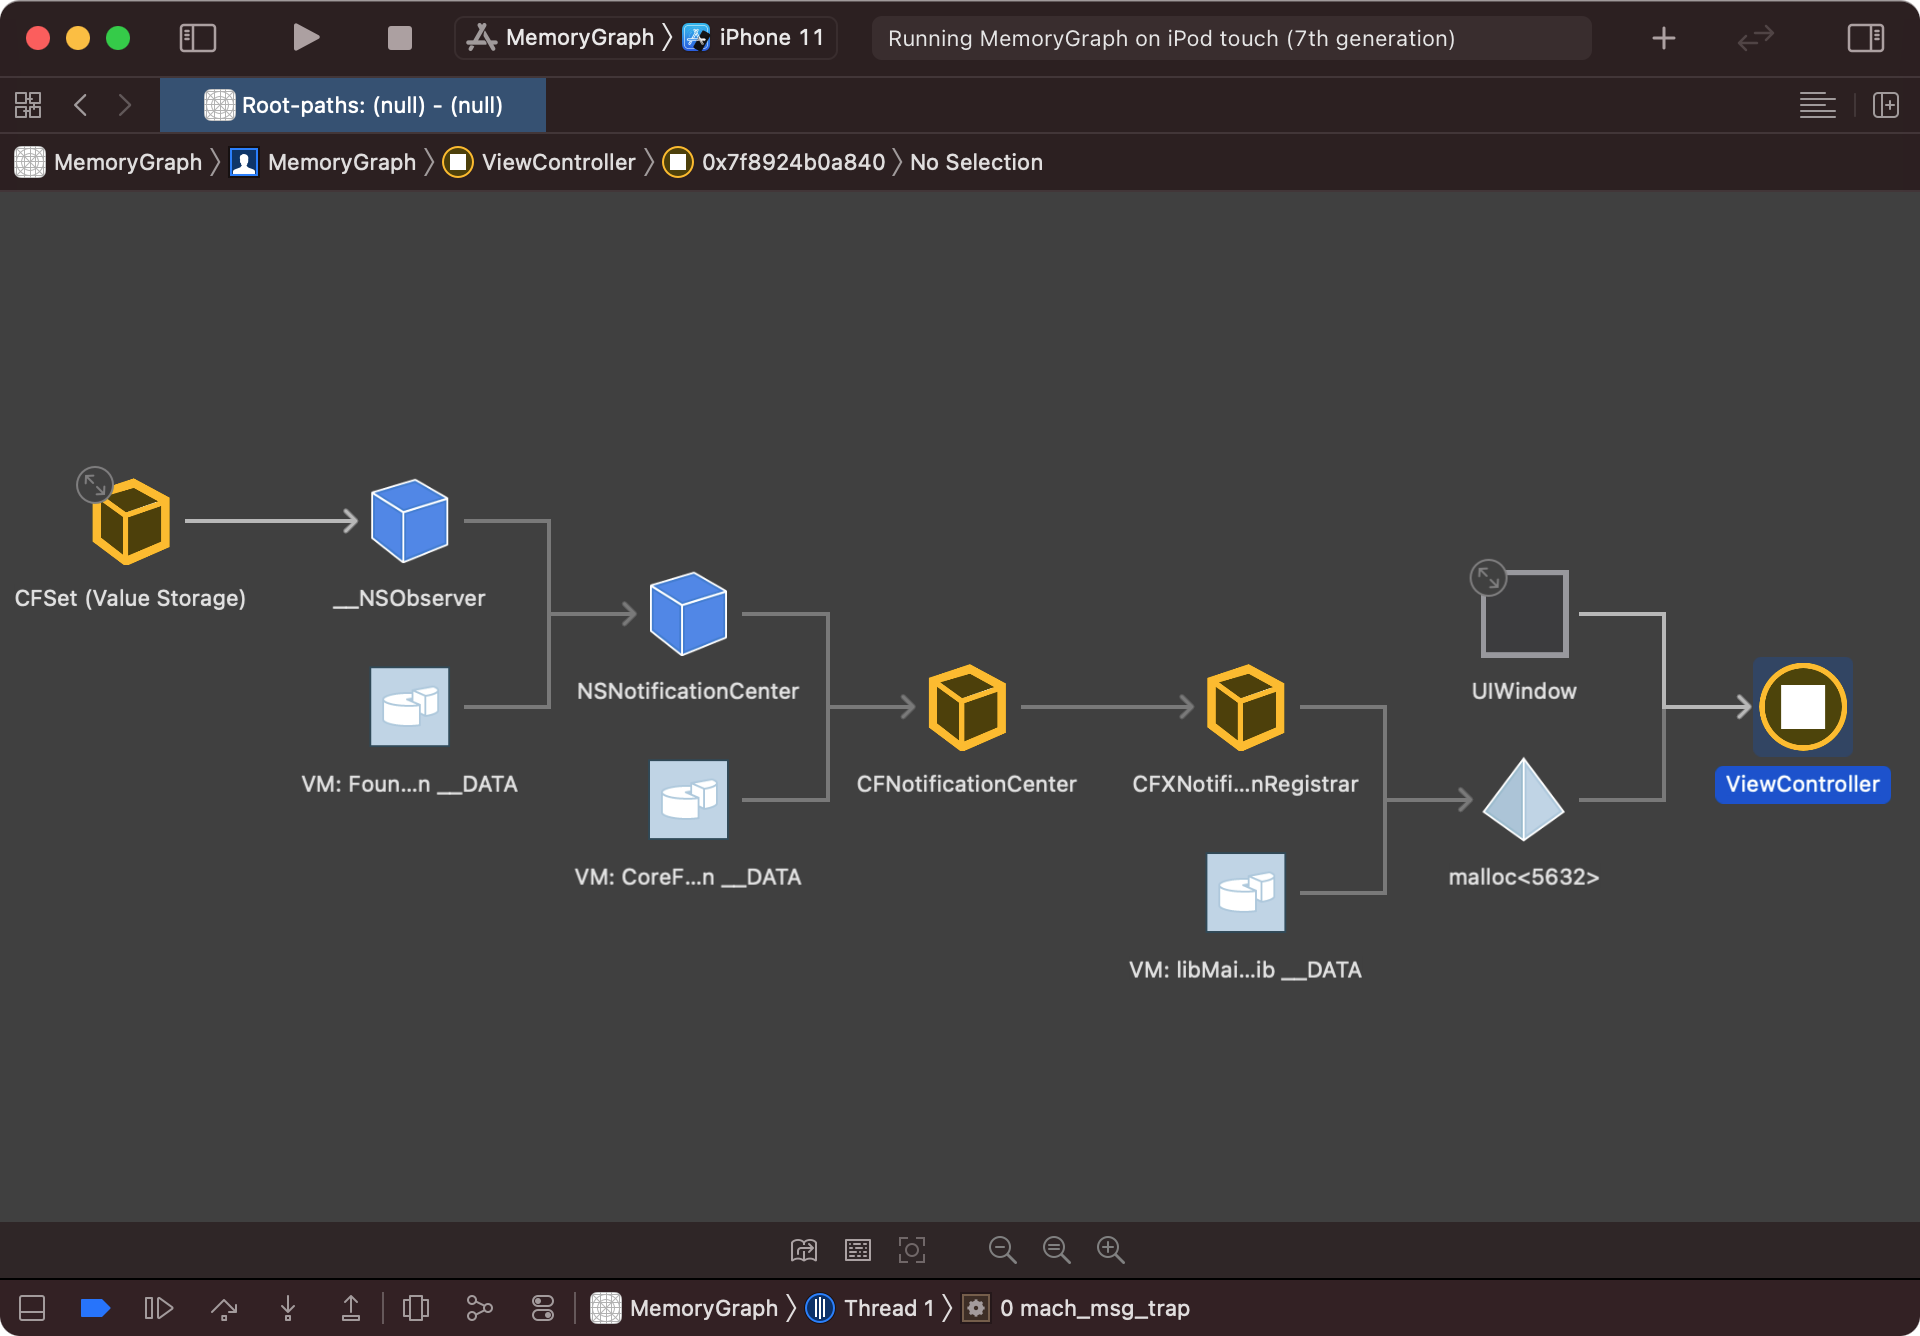
\includegraphics[width=\textwidth]{img/memoryGraph.png}
    \caption{Memory graph in Xcode 12}
\end{figure}


\subsection{Prior Art}
